
\section{Introdução}

O presente relatório tem como objetivo descrever todo o processo implementado durante a resolução do primeiro trabalho prático da UC de Processamento de Linguagem Natural.

O trabalho em causa foi proposto de maneira a serem aplicados, e aprimorados, todos os conhecimentos adquiridos durante as aulas no que se refere ao processamento de documentos PDF.

Com isto, pretende-se extrair a informação com maior relevância, presente nos documentos, de uma forma conveniente, de maneira a assegurar a sua possível utilização em projetos futuros. Para tal, esta informação deve ser armazenada em ficheiros de formato JSON.

Assim sendo, numa primeira parte, serão introduzidos os ficheiros selecionados para processamento, bem como a estrutura definida para os ficheiros JSON finais de cada um. Por forma a alcançar este objetivo final, serão também relatadas todas as etapas de manipulação, envolvendo expressões regulares, de maneira a assegurar uma extração bem sucedida da informação mais relevante.

\section{Pré-requisitos}

Antes de se proceder ao desenvolvimento do projeto em si, certos pré-requisitos, a considerar, consistem em:
\begin{itemize}
    \item Realização do processamento de \textbf{pelo menos 3 ficheiros PDF};
    \item Processamento \textbf{obrigatório} do ficheiro correspondente ao \textbf{Glossário do Ministério da Saúde};
    \item Desenvolvimento do projeto em linguagem \textbf{Python}.
\end{itemize}

\section{Seleção de Ficheiros}
Tal como foi referido anteriormente, para a realização do projeto, devem ser processados, pelo menos, 3 documentos PDF. Tendo isto em conta, e analisando os ficheiros fornecidos para seleção, o grupo decidiu processar os seguintes documentos:

\begin{itemize}
    \item \textbf{Glossário do Ministério da Saúde}, obrigatório;
    \item \textbf{Anatomia na Prática - Sistema Musculoesquelético};
    \item \textbf{Minidicionário de Cardiologista};
\end{itemize}

\subsection{Glossário do Ministério da Saúde}

\subsubsection{Introdução:}
O documento intitulado “Glossário Médico do Ministério da Saúde” é um documento elaborado pelo Ministério da Saúde do Brasil, no ano de 2004, com o objetivo de criar um glossário de vocabulário controlado e de qualidade. 

No que se refere ao conteúdo do documento, e excluindo os segmentos referentes ao Sumário, Apresentação, Introdução, Bibliografia e VCMS, foi possível identificar quatro secções com estruturas diferentes:
\begin{itemize}
    \item Siglas: secção com a lista de siglas utilizadas ao longo do documento e o seu significado;
	\item Glossário: secção majoritária do documento, com os termos e o seu significado, bem como a, ou as, categorias às quais pertence.
	\item Áreas temáticas: secção com todas as categorias referidas no glossário, bem como a sua definição.
	\item Termos organizados por categoria: nesta secção, como o nome indica, para cada categoria existe a lista de termos que nela estão incluídos.
\end{itemize}

\subsubsection{Estrutura de armazenamento definida:}
Por forma a guardar a informação que seria extraída, posteriormente, foram definidos três ficheiros JSON com a seguinte estrutura:

\begin{center}
    \textbf{siglas =}
    \{\textbf{"Sigla":}
    "Significado"\}
\end{center}


\begin{center}
    \textbf{categorias =}
    \{\textbf{"Categoria":}\{
\end{center}
\begin{center}
    \textbf{"Descrição":}
    {Descrição da categoria},
\end{center}
\begin{center}
    \textbf{"Termos":}
    {[Lista de termos]}\}
\end{center}
\}

\begin{center}
    \textbf{glossario =}
    \{\textbf{"Termo":}\{
\end{center}
\begin{center}
    \textbf{"Categoria":}
    {[Lista de categorias]},
\end{center}
\begin{center}
    \textbf{"Definição":}
    {Definição do termo}\}
\end{center}
\}

\subsubsection{Fase 1: Conversão}

De modo a dar início ao processamento e extração da informação do documento, foi essencial convertê-lo de formato pdf para formato xml. Para tal, foi utilizado o comando \textbf{pdftohtml -xml -i}. Este formato foi selecionado devido à sua maior retenção de informação acerca da estrutura do documento, comparativamente ao formato txt.

\subsubsection{Fase 2: Divisão}

Como referido anteriormente, as secções referentes ao Sumário, Apresentação, Introdução, Bibliografia e VCMS foram consideradas desnecessárias para a produção dos ficheiros JSON, acima descritos, e, como tal, foram eliminados, manualmente, do ficheiro xml. \\

Após esta exclusão, os segmentos do ficheiro xml, que correspondem às secções descritas anteriormente, foram dividos em 4 ficheiros xml distintos: \textbf{glossario}, \textbf{misc}, \textbf{categorias} e \textbf{siglas}. Esta divisão adveio do desejo de simplificar o processamento, uma vez que o uso de expressões regulares para processar uma zona do documento poderia prejudicar o processamento de outras. 

\subsubsection{Fase 3: Limpeza}
De modo geral, foi necessário utilizar expressões regulares para eliminar as tags \textbf{text}, \textbf{page}, \textbf{image}, \textbf{itálico} e \textbf{fontspec} dos quatro ficheiros, bem como o número da página.

Para além disso, e especificamente no documento referente ao glossário, foi necessário identificar as expressões regulares que permitem eliminar:
\begin{itemize}
    \item A indicação do primeiro e último termo presentes no cabeçalho de cada página;
    \begin{lstlisting}[style=pythonstyle]
texto = re.sub(r"(</?text.*?></text>\n){2,4}</page>", r"", texto)
\end{lstlisting}
   
    \item A letra do alfabeto à qual se refere cada nova secção do dicionário:
   \begin{lstlisting}[style=pythonstyle]
texto = re.sub(r"</?text.*?>\w</text>", r"", texto)
\end{lstlisting}
\end{itemize}

Por outro lado, no que se refere ao ficheiro misc, os termos que ocupavam mais do que uma linha foram identificados pelo seu alinhamento, parâmetro \textbf{left} da tag \textbf{text}, associado a 4 valores diferentes. Como tal, foi fundamental processar estas situações antes da eliminação das tags text, e proceder à junção dos dois parágrafos que contêm o termo completo. 
\begin{lstlisting}[style=pythonstyle]
texto = re.sub(r'\n<text .*? left="500" .*?>', r'', texto)
texto = re.sub(r'\n<text .*? left="138" .*?>', r'', texto)
texto = re.sub(r'\n<text .*? left="193" .*?>', r'', texto)
texto = re.sub(r'\n<text .*? left="444" .*?>', r'', texto)
\end{lstlisting}

Além disso, o elemento \textbf{new line}, entre cada termo de uma mesma categoria, foi substituído por uma vírgula.
\begin{lstlisting}[style=pythonstyle]
texto = re.sub(r"([^>])\n([^<])", r"\1,\2", texto)
\end{lstlisting}

Por fim, foi necessário proceder à eliminação de duplos espaços, bem como situações de mudança de linha a meio de uma palavra.
\begin{lstlisting}[style=pythonstyle]
texto = re.sub(r"- ", r"", texto)
texto = re.sub(r"  ", r" ", texto)

\end{lstlisting}

\subsubsection{Fase 4: Extração e Construção do dicionário final}

\textbf{Ficheiro siglas:}

Após a limpeza do documento, a informação restante está limitada a cada sigla, inserida numa tag \textbf{bold}, seguida do seu significado. Como tal, para extrair a sigla e o seu significado, foi utilizada a expressão:
\begin{lstlisting}[style=pythonstyle]
<b>(.+?)</b>([^<]+)
\end{lstlisting}
O tuplo resultante foi convertido num dicionário, com a estrutura definida previamente.
Este dicionário foi guardado no ficheiro JSON “siglas.json”.
\begin{figure}[H]
    \centering
    \centering
    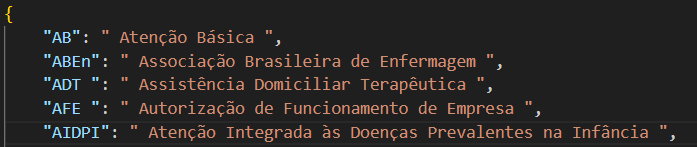
\includegraphics[width=0.8\textwidth]{Images/dic_siglas.png}
    \caption{Dicionário siglas}
    \label{fig:exemplopag}
\end{figure}

\textbf{Ficheiro misc:}

De forma semelhante, o ficheiro misc, após a limpeza, possuía apenas o nome de cada categoria rodeado pela tag \textbf{bold}, b, e a lista de termos que contém, pelo que foi utilizada a mesma expressão para extrair a informação. \\
Para além disso, foi utilizado um ciclo \textbf{for} para construir o dicionário cujas chaves correspondem às categorias, primeiro elemento do tuplo resultante do findall. Por sua vez, os valores destas chaves correspondem às listas resultantes da utilização do método split, aplicado ao segundo elemento do tuplo, pelo separador “,”. Este dicionário irá ser utilizado como auxiliar na construção de um outro, numa fase posterior, não tendo sido, portanto, mencionado anteriormente. 

O dicionário produzido foi guardado no ficheiro “misc.json”.

\textbf{Ficheiro categorias:}

Novamente, após a etapa anterior, o ficheiro categorias continha apenas o nome de cada categoria rodeado pela tag bold, b, e a sua definição, pelo que foi utilizada a expressão já mencionada para extrair a informação. 

No entanto, para construir o dicionário com a estrutura desejada, foi necessário carregar o dicionário criado a partir do ficheiro misc, designado termos\_categoria. Deste modo, e utilizando um ciclo for, fez-se a correspondência entre cada categoria, primeiro elemento do tuplo resultante da função findall, e um novo dicionário. Este dicionário tem como chaves as palavras “Definição” e “Termos”, cujos valores são, respetivamente, o segundo elemento do tuplo e o valor, com a mesma chave, do dicionário termos\_categoria. 
\begin{figure}[H]
    \centering
    \centering
    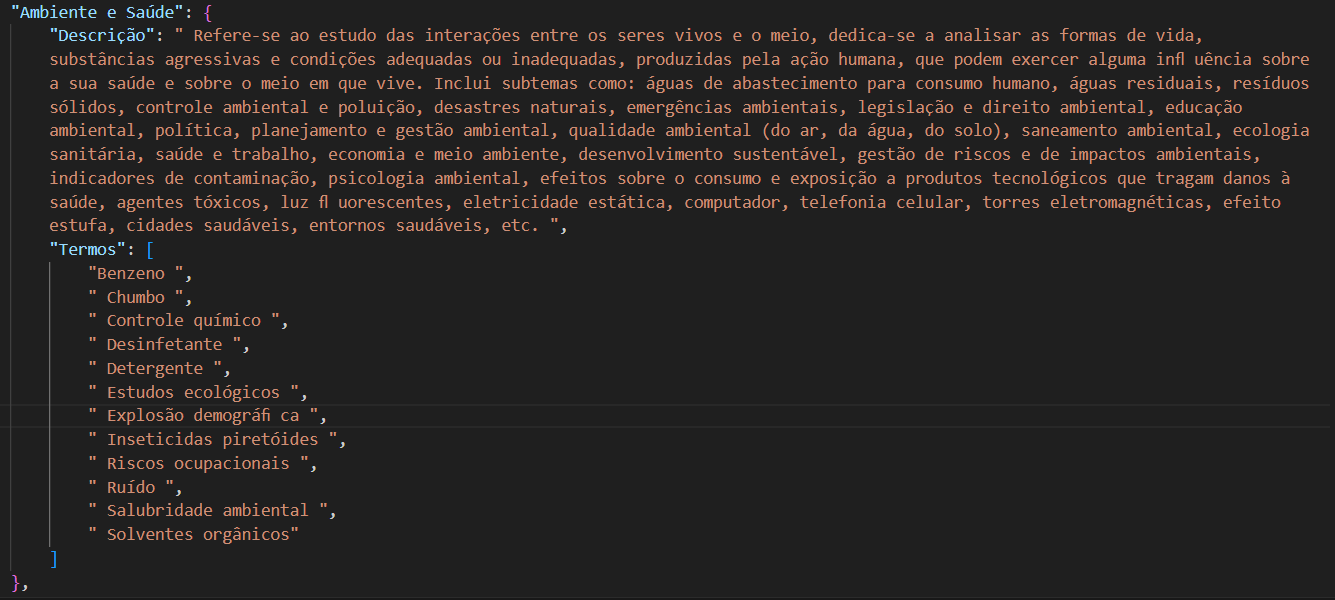
\includegraphics[width=1.0\textwidth]{Images/categorias.png}
    \caption{Dicionário categorias}
    \label{fig:exemplopag}
\end{figure}

\textbf{Ficheiro glossario:}

Antes da limpeza do ficheiro, o documento foi analisado com o objetivo de encontrar padrões para facilitar a extração da informação, e apesar das designações estarem rodeadas pela tag bold, b, não existe distinção entre o texto referente às categorias e a definição do termo.

Como tal, após a limpeza, foram iteradas as chaves do dicionário construído a partir do ficheiro categorias, e em todas as ocorrências das mesmas, no ficheiro glossário, foi adicionado o elemento @ no início e no fim da categoria. 

No entanto, a categoria “Doenças” não possui correspondência direta com as chaves do dicionário, uma vez que, e como é explicado no próprio documento, esta categoria agrega doenças para além das “Doenças Crônicas e Degenerativas” e "Doenças Infeciosas e Parasitárias". Deste modo, foi necessário que a sua identificação e marcação fosse feita utilizando duas expressões regulares específicas.\\

\begin{lstlisting}[style=pythonstyle]
texto = re.sub("Categoria: Doenças", "Categoria: @Doenças@", texto)
texto = re.sub("@  Doenças", "@ @Doenças@", texto)
\end{lstlisting}

Após a marcação das categorias, procedeu-se à marcação dos casos em que existiam mais de uma categoria, num mesmo termo. Para tal, substitui-se a ocorrências de dois “@” seguidos, que representam o fim de uma categoria e início de outra, por um elemento “\&”.

Após estas adições foi possível utilizar a seguinte expressão regular: 
\begin{lstlisting}[style=pythonstyle]
<b>([\^<]+?)</b> Categoria: @(.+?)@([\^<]+)
\end{lstlisting}
Esta permite extrair os conceitos, com o primeiro elemento do tuplo a corresponder ao termo, o segundo à categoria ou categorias, e o último à definição do conceito.

Para a construção do dicionário desejado, dic\_termos, foi utilizado um ciclo for, de forma a iterar pelas instâncias extraídas pela função findall, para fazer a correspondência entre cada valor do primeiro elemento do tuplo, e novo dicionário, cujas chaves são “Categoria” e “Definição. Os valores que correspondem a estas chaves, são respetivamente, a lista resultante do método split, pelo separador “\&”, aplicado ao segundo elemento do tuplo e o último elemento deste.

Por outro lado, também se verificou que nem todos os termos possuem categoria e descrição, alguns deles apenas fazem referência a um outro termo, por exemplo, \textbf{<b>Didanosina</b> Ver DDI}. Como tal, foi necessário definir uma expressão regular, para a extração da informação, distinta da utilizada para os termos com estrutura comum:
\begin{lstlisting}[style=pythonstyle]
<b>([^<]+)</b> (Ver [^<]+)
\end{lstlisting}

Estes conceitos foram adicionados ao dicionário dic\_termos, utilizando novamente um ciclo for, que permitiu criar uma entrada, cuja chave é o primeiro elemento do tuplo e o valor o segundo. Por fim, este dicionário foi ordenado de forma que as suas chaves estivessem organizadas alfabeticamente.

\begin{figure}[H]
    \centering
    \centering
    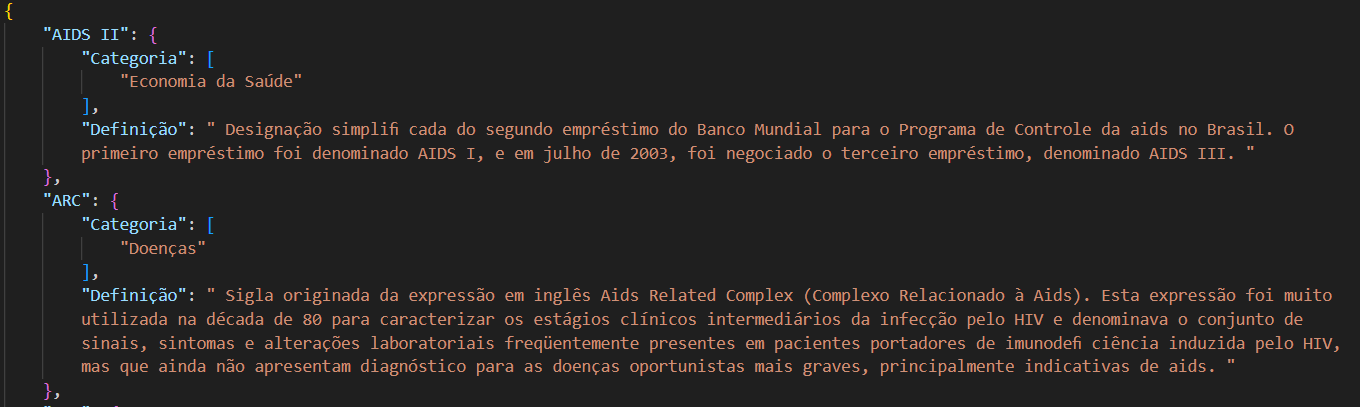
\includegraphics[width=1.0\textwidth]{Images/glossario.png}
    \caption{Dicionário glossario}
    \label{fig:exemplopag}
\end{figure}

\subsection{Anatomia na Prática - Sistema Musculoesquelético}

\subsubsection{Introdução:}

Tal como o nome indica, o ficheiro em causa trata-se de um documento que permite colocar em prática o conhecimento da anatomia humana, mais especificamente do sistema musculoesquelético, de estudantes de Medicina.

Em termos de conteúdo, numa parte inicial, é possível averiguar a presença de uma breve descrição dos autores, e tema do documento, bem como um índice/sumário em que é estabelecida uma enumeração das principais secções do documento.

Tendo em conta que o foco do ficheiro se trata do auxílio ao estudo da anatomia humana, verifica-se que a maioria deste é composto por imagens, em conjunto com alíneas, sendo estas usadas para identificar determinadas partes do corpo humano.
Assim, o aluno, durante a resolução dos exercícios, para cada alínea, toma nota da nomenclatura do componente anatómico em causa, podendo dirigir-se à secção final do documento para comparar as suas respostas.


É ainda importante realçar a divisão do documento em diversas secções e subsecções:
\begin{itemize}
    \item Mais especificamente, verificam-se \textbf{dois grandes grupos}: o \textbf{Sistema Esquelético e Articular} e o \textbf{Sistema Muscular}.

    \item Seguidamente, para cada sistema global, averiguam-se várias secções devidamente numeradas, como \textbf{1. Crânio}, \textbf{2. Membro Superior}, \textbf{3. Membro Inferior}, etc.

    \item Por sua vez, cada secção em si, verifica múltiplas subsecções. Por exemplo, relativamente à secção \textbf{1. Crânio}, surgem as subsecções \textbf{1.1 Crânio: Vista Anterior - I}, \textbf{1.2 Crânio: Vista Anterior - II}, etc. Consequentemente, é cada subsecção que apresenta as mais diversas nomenclaturas associadas.

    \item No entanto, é de capital importância denotar que algumas subsecções poderão apresentar, também, outras secções, como é o caso de \textbf{4.4 Vértebras Cervicais Atípicas: Áxis (C2) - Vista Póstero-Superior} e 
    \textbf{4.4.1 Vista Lateral}, sendo que é nesta última que se averiguam as diferentes terminologias.

\end{itemize}
 
\begin{figure}[H]
    \centering
    \centering
    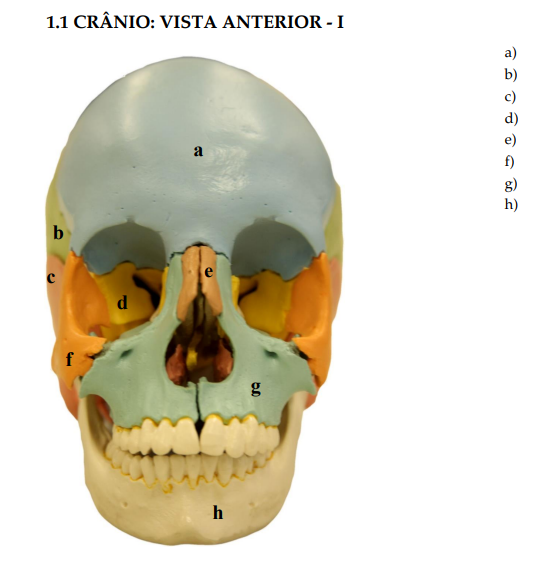
\includegraphics[width=0.5\textwidth]{Images/exemplopag.png}
    \caption{Exemplo de uma das páginas do documento}
    \label{fig:exemplopag}
\end{figure}

\subsubsection{Estrutura de armazenamento definida:}

Posto isto, uma vez que a informação mais relevante, no que diz respeito a este documento, se trata da nomenclatura dos mais diversos elementos anatómicos, decidiu-se implementar um dicionário, posteriormente armazenado no ficheiro JSON, com a seguinte estrutura:

\begin{center}
    \textbf{dicionário =}
\end{center}
\textbf{\{}
\begin{center}
    \textbf{"SISTEMA ESQUELÉTICO E ARTICULAR":}
    \{"SECÇÃO1":
\end{center}

\begin{center} 
    \{"SUBSECÇÃO1": [terminologia1, terminologia2, terminologia3, ...],
\end{center}

\begin{center}
    "SUBSECÇÃO2": \{\texttt{"SUB\_SUBSECÇÃO1":} [terminologia1, terminologia2, ...]\}\}\}
\end{center}

\\
\begin{center}
    \textbf{"SISTEMA MUSCULAR":}
    \{"SECÇÃO1":
\end{center}

\begin{center} 
    \{"SUBSECÇÃO1": [terminologia1, terminologia2, terminologia3, ...],
\end{center}
    
\begin{center}
    "SUBSECÇÃO2": \{\texttt{"SUB\_SUBSECÇÃO1":} [terminologia1, terminologia2, ...]\}\}\}
\end{center}
\textbf{\}}

Assim, basta apenas procurar pela subsecção desejada para averiguar as diferentes terminologias associadas.

\subsubsection{Fase 1: Conversão}
De maneira a dar início ao processo de preparação e limpeza do documento, por forma a dar origem ao ficheiro JSON final, o mesmo foi submetido a uma conversão para o formato \textbf{xml}.

Esta decisão reside no facto de a linguagem xml permitir uma maior facilidade de identificação de padrões uma vez que organiza os dados numa estrutura hierárquica, através do uso de tags, que, por sua vez, apresentam nomes descritivos, que auxiliam o ser humano na compreensão do conteúdo.


\subsubsection{Fase 2: Limpeza}
\textbf{Eliminação Manual:}
Tal como foi referido anteriormente, a informação relevante, a ser extraída, diz respeito às respostas, presentes na secção final do documento, referentes às diferentes nomenclaturas dos componentes.

Esta secção diz respeito à secção \textbf{Gabarito}, que se inicia a partir da página 192 do documento. Posto isto, após abertura do documento, já em formato xml, no editor de texto, qualquer conteúdo presente acima desta secção foi eliminado.

\textbf{Expressões Regulares:}\\
No que diz respeito às expressões regulares, estas assumíram um papel bastante importante na fase de limpeza, uma vez que permitiram eliminar padrões específicos, que se repetiam continuamente ao longo do documento.

Um exemplo prático desta situação consiste no menu vertical, vigente em todas as páginas, pelo que se revelou necessário utilizar a função \textbf{sub} das RegEx, de maneira a proceder à sua eliminação.

A identificação do seu respetivo padrão não foi difícil, uma vez que constituíam as únicas tags de texto com fontes correspondentes a 4 e a 5. 

\begin{figure}[H]
    \centering
    \centering
    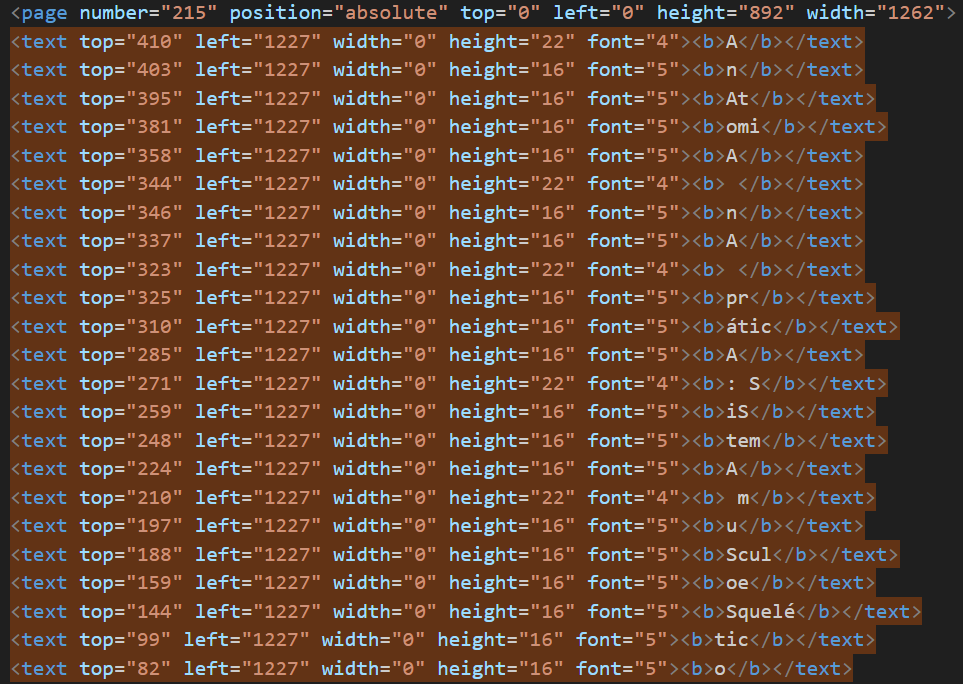
\includegraphics[width=0.6\textwidth]{Images/menu_vertical.png}
    \caption{Menu Vertical - identificação}
    \label{fig:desccortada}
\end{figure}

Para além disso, as expressões regulares foram também utilizadas para descartar outro tipo de conteúdo, como:
\begin{itemize}
    \item As \textbf{page tags};
    \begin{lstlisting}[style=pythonstyle]
text = re.sub(r"</page>\n<page.+>(\n)+", r"", text) 
\end{lstlisting}
    
    \item As tags correspondentes a \textbf{elementos âncora};
    \begin{lstlisting}[style=pythonstyle]
text = re.sub(r".+<a.+\n.+", r"", text) 
\end{lstlisting}
    
    \item Os números, delimitados pelas tags bold, uma vez que se tratavam dos \textbf{números das páginas};
    \begin{lstlisting}[style=pythonstyle]
text = re.sub(r".+<b>\d+</b>.+\n+", r"", text)
\end{lstlisting}

    \item As \textbf{text tags}, juntamente com os mais diversos parâmetros, isto é font, width, height, etc.
    \begin{lstlisting}[style=pythonstyle]
text = re.sub(r"</?text.*?>", r"", text) 
\end{lstlisting}
\end{itemize}

\subsubsection{Fase 3: Correção de anomalias}
\textbf{Subsecções}:\\
Uma vez obtida uma melhor identificação do conteúdo a ser extraído, foi importante proceder a uma análise de quaisquer anomalias a serem corrigidas.

Por exemplo, enquanto que determinadas subsecções se encontravam delimitadas pelas tags bold, numa única linha, outras, ou não se encontravam a bold, ou, então, a sua designação continuava numa linha posterior:

\begin{figure}[H]
    \centering
    \centering
    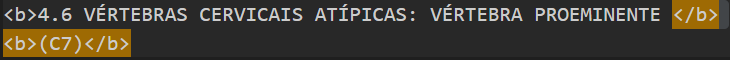
\includegraphics[width=0.7\textwidth]{Images/C7.png}
    \caption{Subsecções anómalas - continuação da descrição numa nova linha}
    \label{fig:c7}
\end{figure}

\begin{figure}[H]
    \centering
    \centering
    \includegraphics[width=0.4\textwidth]{Images/descriçãocortada.png}
    \caption{Subsecções anómalas - continuação da descrição numa nova linha}
    \label{fig:desccortada}
\end{figure}

\begin{figure}[H]
    \centering
    \centering
    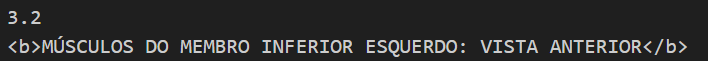
\includegraphics[width=0.7\textwidth]{Images/seccaosembold.png}
    \caption{Subsecções anómalas}
    \label{fig:sembold}
\end{figure}

É possível concluir, portanto, que o padrão, normal, identificador das \textbf{subsecções} corresponde a:
\begin{center}
    \textbf{<b> n.n Designação </b>} sendo n um número inteiro
\end{center}

Por último, constatou-se a presença de mais uma anomalia, no que se refere às subsecções, mais concretamente das subsecções \textbf{1.25} e \textbf{1.26}, pertencentes ao Sistema Esquelético e Articular, dado que não apresentam quaisquer nomenclaturas associadas:

\begin{figure}[H]
    \centering
    \centering
    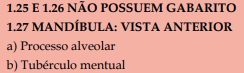
\includegraphics[width=0.4\textwidth]{Images/gabarito.png}
    \caption{Subsecções sem terminologias}
    \label{fig:sembold}
\end{figure}
A decisão final consistiu na sua simples remoção, através da seguinte expressão regular:
\begin{lstlisting}[style=pythonstyle]
text = re.sub(r"\n<b>1.25.+</b>", r"", text)
\end{lstlisting}

\textbf{Terminologias}:\\
No que se refere às terminologias dos respetivos elementos anatómicos, foi possível concluir que estas assumem a seguinte estrutura:
\begin{center}
    \textbf{x) Nome do componente}
\end{center}
No entanto, é importante notar que x pode corresponder a:
\begin{itemize}
    \item uma letra \textbf{minúscula}, ou \textbf{maiúscula}, seguida de um \textbf{parênteses: a)};

    \item uma letra \textbf{minúscula}, seguida de um \textbf{espaço} e \textbf{parênteses: f )};

    \item um \textbf{par letra número}, seguido de \textbf{parênteses}, como por exemplo: \textbf{d1)}.
\end{itemize}

Em termos de anomalias, foi possível observar que uma das terminologias não apresentava um parênteses a seguir à respetiva letra:

\begin{figure}[H]
    \centering
    \centering
    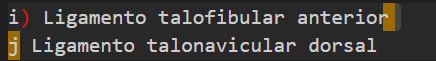
\includegraphics[width=0.5\textwidth]{Images/alineasemparenteses.png}
    \caption{Terminologia anómala}
    \label{fig:semparenteses}
\end{figure}
Para tal, foi utilizada uma expressão regular específica por forma a gerar a estrutura desejada:
\begin{lstlisting}[style=pythonstyle]
text = re.sub(r"\nj\s", r"\nj) ", text)
\end{lstlisting}

Seguidamente, averiguou-se a \textbf{presença de múltiplas terminologias numa única linha}:

\begin{figure}[H]
    \centering
    \centering
    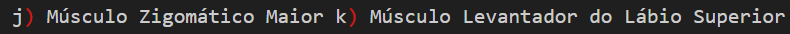
\includegraphics[width=0.8\textwidth]{Images/alinea_mesmalinha.png}
    \caption{Terminologias numa única linha}
    \label{fig:mesmalinha}
\end{figure}
Na imagem acima, as alíneas são constituídas por uma letra, seguida de um parênteses, contudo, foi também possível averiguar o mesmo caso para alíneas de formato letra+número, seguidos de parênteses, como também para alíneas de formato letra+espaço, seguidos de parênteses.

Por forma a contornar esta situação, foram utilizadas expressões regulares, para cada caso específico, uma vez que não foi possível estabelecer uma generalização. Tal decisão pode ser justificada pelo facto de determinadas alíneas poderem ser antecipadas, ou por letras, ou por espaços, o que complicava o processo de generalização.

Abaixo encontram-se listadas as expressões regulares que permitiram contornar estas situações:
\begin{lstlisting}[style=pythonstyle]
text = re.sub(r"\s([a-z]\))", r"\n\1", text) #alíneas letra+parênteses
text = re.sub(r"([a-z\)])(([a-z]\d)\))", r"\1\n\2", text) #alíneas letra+número
text = re.sub(r"([a-z]\s\))", r"\n\1", text) #alíneas letra+espaço
\end{lstlisting}

Em contrapartida, no que se refere à nomenclatura propriamente dita, determinados conceitos encontravam-se \textbf{separados por uma nova linha} e delimitados, ou pelas \textbf{tags bold}, ou pelas \textbf{tags itálico}.

Esta situação é passível de constatar relativamente a \textbf{tíbia}, \textbf{tálus} e \textbf{Fascia Transversalis} como é possível observar na imagem abaixo:

\begin{figure}[H]
    \centering
    \centering
    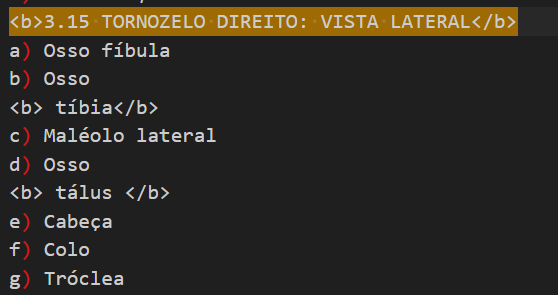
\includegraphics[width=0.6\textwidth]{Images/termosabold.png}
    \caption{Terminologias entre tags bold}
    \label{fig:termosbold}
\end{figure}

\begin{figure}[H]
    \centering
    \centering
    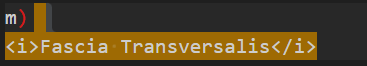
\includegraphics[width=0.4\textwidth]{Images/termo_italico.png}
    \caption{Terminologia entre tags itálico}
    \label{fig:termositalico}
\end{figure}

De maneira a corrigir estas anomalias, procedeu-se à eliminação das tags, e posterior retorno para a linha anterior, através do uso da função \textbf{sub} das RegEx.\\
A linha abaixo demonstra a expressão regular empregue para o caso da terminologia \textbf{Fascia Transversalis:}
\begin{lstlisting}[style=pythonstyle]
text = re.sub(r"\n<i>(.+)</i>", r"\1", text)   
\end{lstlisting}


\subsubsection{Fase 4: Sintaxe de extração definida}

Dada por concluída a fase de correção de anomalias, em que é possível observar os diferentes padrões distintivos de cada componente, isto é dos dois grupos globais, das secções e subsecções, e terminologias, a fase seguinte consiste na definição de uma sintaxe, própria para cada um, de maneira a facilitar o processo de extração pela função \textbf{findall} das RegEx.

Posto isto, foi definido que:

\begin{itemize}
    \item Os dois grandes grupos, isto é, \textbf{Sistema Esquelético e Articular} e \textbf{Sistema Muscular} são antecipados pelo símbolo \textbf{\&};
    \begin{lstlisting}[style=pythonstyle]
text = re.sub(r"<b>([^\d]+)</b>", r"&\1", text)
\end{lstlisting}

    \item As \textbf{secções} são antecipadas pelo símbolo \textbf{\%};
    \begin{lstlisting}[style=pythonstyle]
text = re.sub(r"<b>\d\.?\s?([A-Z\sÂÓÁÉÊÔÚÇ]+)</b>", r"%\1", text)
\end{lstlisting}

    \item As \textbf{subsecções} são antecipadas pelo símbolo \textbf{\#};
    \begin{lstlisting}[style=pythonstyle]
text = re.sub(r"<b>\d\.\s?\d+\.?\s?(.+)</b>", r"#\1", text)
\end{lstlisting}

    \item As \textbf{terminologias} são antecipadas pelo símbolo \textbf{@};
    \begin{lstlisting}[style=pythonstyle]
text = re.sub(r"\n(([a-z]\s?\))|(([a-z][0-9])\s?\))|([A-Z]\s?\)))", r"\n@", text)
\end{lstlisting}

    \item As eventuais \textbf{secções} de \textbf{subsecções} são antecipadas pelo símbolo \textbf{;}.
    \begin{lstlisting}[style=pythonstyle]
text = re.sub(r"<b>\d\.\d\.\d\.?\s?(.+)</b>", r";\1", text) 
\end{lstlisting}
\end{itemize}

Todo este processo facilitou a extração de todos estes diferentes elementos para as suas respetivas listas, de maneira a ser possível implementar o código de construção do dicionário final.

\subsubsection{Fase 5: Construção do dicionário final}

De um modo geral, o raciocínio de construção do dicionário final consistiu em:

\begin{itemize}
    \item Escrita, num ficheiro \textbf{txt}, do conteúdo final do documento, já corrigido e com a sintaxe anteriormente definida;
    
    \item Definição de um dicionário, \textbf{dic}, vazio, para armazenar os dados analisados do ficheiro anterior;

    \item Definição de variáveis de controlo como \texttt{cur\_titulo}, \texttt{cur\_seccao}, \texttt{cur\_subseccao} \\
    e \texttt{cur\_sub\_subseccao}, inicializadas como None;

    \item \textbf{Abertura} do ficheiro txt para leitura, sendo o seu conteúdo dividido em linhas;

    \item \textbf{Iteração} sobre cada linha;

    \item Para cada linha, \textbf{verificar} se o texto, sem o primeiro caractere, dado que não se pretende incluir os símbolos definidos anteriormente, está presente numa das listas resultantes do \textbf{findall}. Isto é, pretende-se averiguar se se trata de uma secção, subsecção, etc;

    \item Dependendo de onde a linha se encaixa, a \textbf{variável de controlo}, correspondente, é \textbf{atualizada};

    \item Quando uma \textbf{linha começa com "@"} (indicando uma nomenclatura), esta é \textbf{adicionada ao dicionário}, no nível apropriado da hierarquia de seções;

    \item Após iterar por todas as linhas, o dicionário dic é \textbf{convertido em formato JSON};

    \item O ficheiro final designa-se \textbf{"dicionario.json"} com codificação UTF-8 e formato de indentação de 4 espaços.

\end{itemize}

As imagens abaixo permitem observar partes do resultado final:

\begin{figure}[H]
    \centering
    \centering
    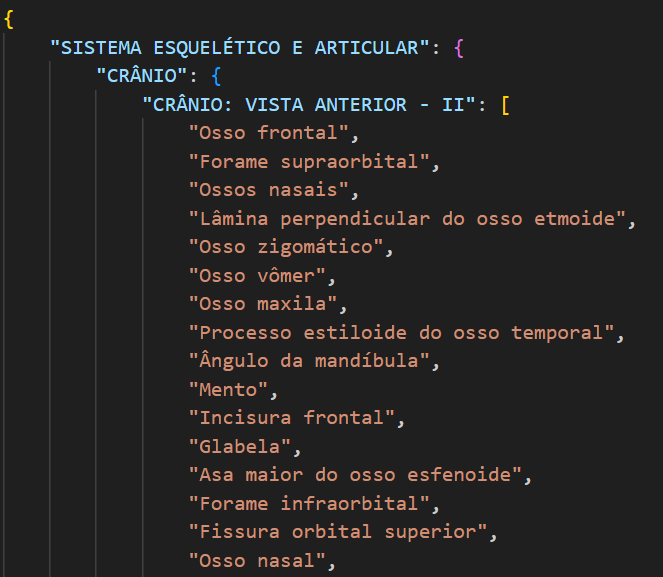
\includegraphics[width=0.7\textwidth]{Images/final1.png}
    \caption{Parte inicial do dicionário final}
    \label{fig:final1}
\end{figure}

\begin{figure}[H]
    \centering
    \centering
    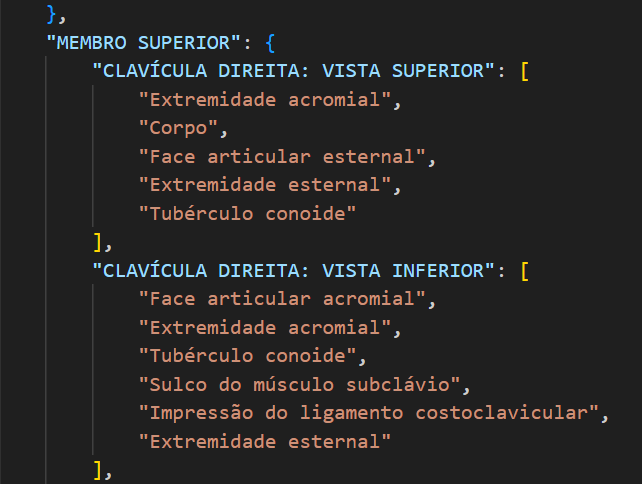
\includegraphics[width=0.7\textwidth]{Images/final2.png}
    \caption{Parte intermédia do dicionário final}
    \label{fig:final2}
\end{figure}

Exemplo de subsecções com secções:
\begin{figure}[H]
    \centering
    \centering
    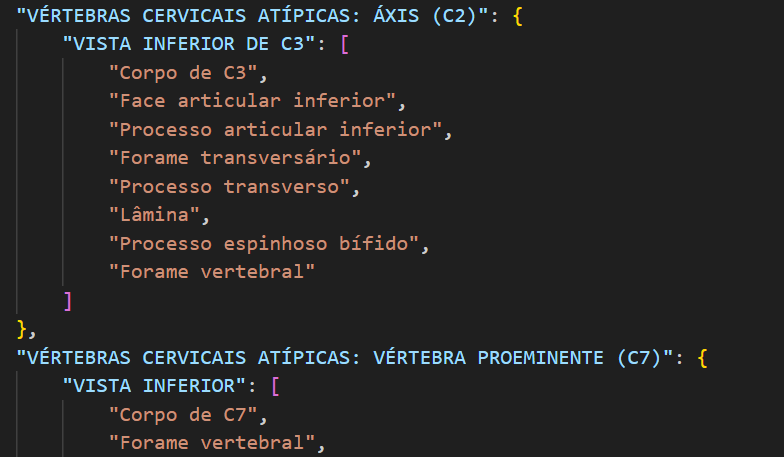
\includegraphics[width=0.8\textwidth]{Images/final3.png}
    \caption{Caso de subsecções com secções}
    \label{fig:final3}
\end{figure}

\subsection{Minidicionário de Cardiologista}

\subsubsection{Introdução:}

O ficheiro em questão trata-se de um dicionário Inglês-Português e Português-Inglês das expressões, e termos mais frequentes, em escala mundial, no âmbito da Cardiologia. 

Em relação ao conteúdo, numa parte inicial, são encontradas as secções referentes à apresentação, à breve descrição do autor, bem como aos agradecimentos. Em seguida, o documento é dividido em duas grandes secções: a primeira apresenta os termos e expressões em Inglês, com as suas respetivas traduções para Português; a segunda, o oposto. O ficheiro termina, por sua vez, com as referências bibliográficas utilizadas pelo autor durante o desenvolvimento do dicionário.

\begin{figure}[H]
    \centering
    \begin{subfigure}{0.4\textwidth}
      \centering
      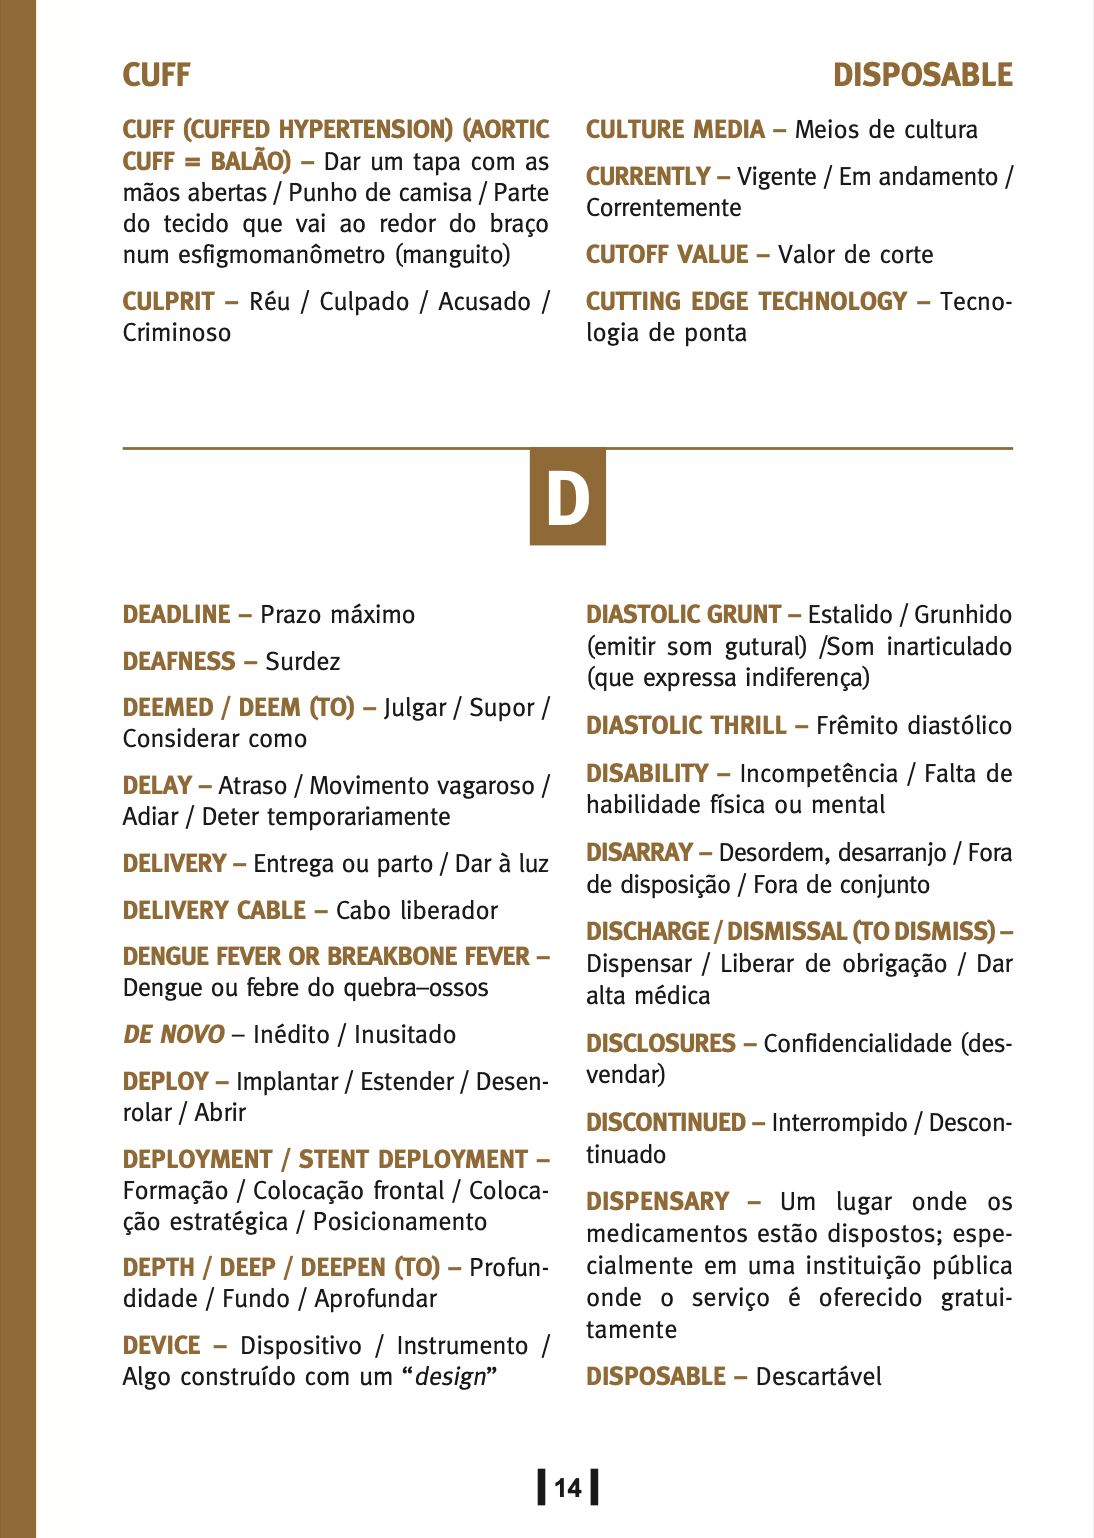
\includegraphics[width=\textwidth]{Images/ingles-portugues.png}
      \caption{Exemplo de uma página da secção Inglês-Português}
      \label{fig:ingles-portugues}
    \end{subfigure}
    \hfill
    \begin{subfigure}{0.4\textwidth}
      \centering
      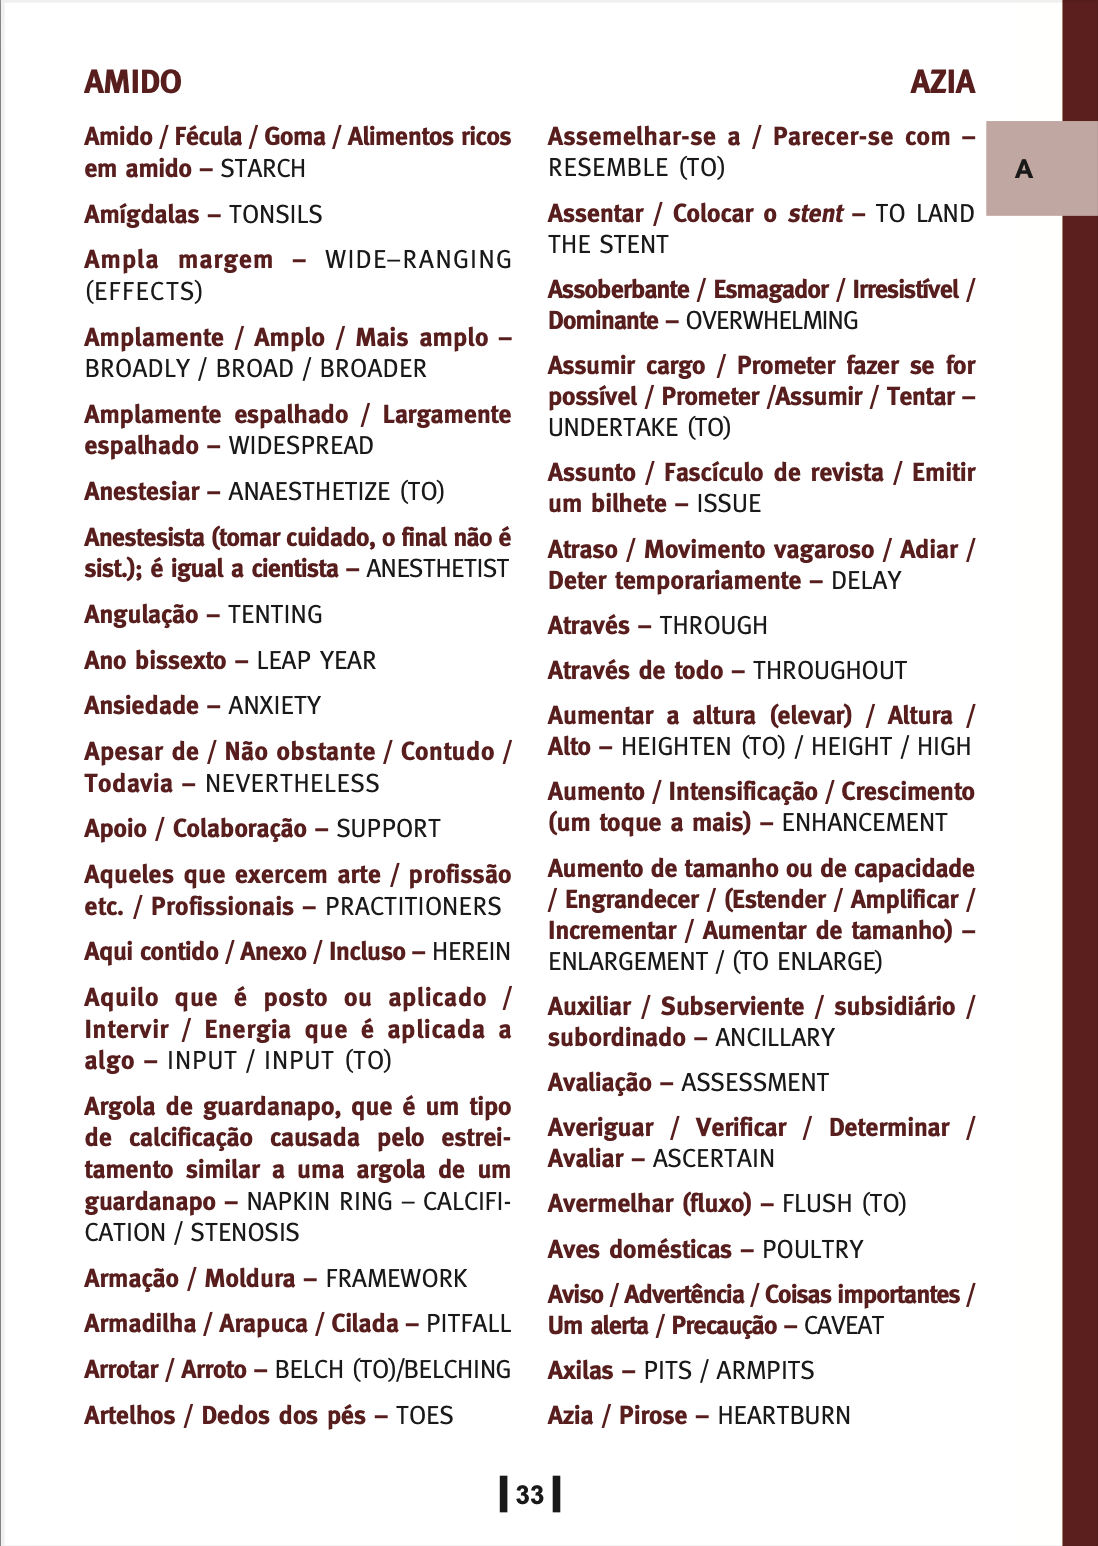
\includegraphics[width=\textwidth]{Images/portugues-ingles.png}
      \caption{Exemplo de uma página da secção Português-Inglês}
      \label{fig:portugues-ingles}
    \end{subfigure}
    \caption{Secções do Minidicionário de Cardiologista}
    \label{fig:seccoes}
\end{figure}

\subsubsection{Estrutura de armazenamento definida:}

De acordo com o reconhecimento das duas grandes secções no documento em estudo, decidiu-se implementar um dicionário, posteriormente armazenado num ficheiro JSON, com a seguinte estrutura:

\begin{center}
    \textbf{dic\_traduc =}
    \textbf{\{}
\end{center}
\begin{center}
    \textbf{"ingles-portugues":}
    \{"termo1": "traducao1", "termo2: "traducao2", ...\}
\end{center}

\begin{center}
    \textbf{"portugues-ingles":}
   \{"termo1": "traducao1", "termo2: "traducao2", ...\}
   \textbf{\}}
\end{center}

\subsubsection{Fase 1: Conversão}
Para iniciar o processo de preparação e limpeza do documento, com o objetivo de gerar o ficheiro JSON final, optou-se por converter o documento para o formato \textbf{xml}. 

Esta escolha baseia-se na capacidade da linguagem xml facilitar a identificação de padrões, uma vez que organiza os dados numa estrutura hierárquica por meio do uso de tags que, por sua vez, possuem nomes descritivos que auxiliam na compreensão do conteúdo.

\subsubsection{Fase 2: Limpeza e Extração}

\textbf{Eliminação Manual:}
Conforme estabelecido anteriormente, as partes iniciais e finais do documento não apresentam informações relevantes sobre os termos e as suas respetivas traduções. Portanto, todo o conteúdo no ficheiro, em formato xml, acima da página 9 (inicío da secção Inglês-Portugal) e abaixo da página 51 (fim da secção Português-Inglês) foi eliminado. 

\textbf{Expressões Regulares:}
Através da estrutura do ficheiro em formato xml foi possível identificar padrões referentes aos termos e às suas traduções que facilitaram a limpeza e a extração.

Em relação à secção Inglês-Português, foi possível observar que os termos apresentavam, dentro da tag \textbf{<text>}, a propriedade \textbf{font="7"} e que, além disso, estavam dispostos entre tags \textbf{<b>}. Logo, através do uso da função \textbf{sub} das RegEx foi possível sinalizar o início e o fim dos termos com o símbolo \textbf{@} a fim de facilitar a posterior extração. 

\begin{lstlisting}[style=pythonstyle]
line = re.sub(r'font="7"><b>(.+?)(</b>.*)',r'font="7"><b>@\1\2', line)
\end{lstlisting}

De igual forma, para a secção Português-Inglês, o mesmo padrão foi observado, no entanto, verificou-se uma diferença sútil na função \textbf{<text>} em que a propriedade \textbf{font} apresentava um valor igual a 13.

\begin{lstlisting}[style=pythonstyle]
line = re.sub(r'font="13"><b>(.+?)(</b>).*',r'font="13"><b>@\1\2', line)
\end{lstlisting}

Após as devidas sinalizações, utilizou-se a função \textbf{findall} das RegEx para extrair todos os termos presentes no documento e armazená-los numa lista denominada \textbf{lista\_termo}.

\begin{lstlisting}[style=pythonstyle]
termos = re.findall(r'(<b>@[^@]+@</b>)', text)
\end{lstlisting}

\begin{lstlisting}[style=pythonstyle]
result = re.findall(r'<b>(.*?)</b>', t)
\end{lstlisting}

Em relação às traduções, o mesmo padrão foi observado nas duas secções: a tag \textbf{<text>} apresentava a propriedade \textbf{font="8"} e não estavam dispostas entre tags \textbf{<b>}. Sendo assim, utilizou-se o mesmo mecanismo para extrair os termos, e respetivas traduções, pelo que foram armazenados numa lista chamada \textbf{lista\_traducoes}.

\begin{lstlisting}[style=pythonstyle]
line = re.sub(r'font="8">(.+?)(.*)</text>',r'font="8">\1\2@</text>', line)
\end{lstlisting}

\begin{lstlisting}[style=pythonstyle]
traducoes = re.findall(r'(font="8">@[^@]+@</text>)', text)
\end{lstlisting}

\begin{lstlisting}[style=pythonstyle]
result = re.findall(r'>(.*)</text>', trad)
\end{lstlisting}

\begin{figure}[H]
    \centering
    \begin{subfigure}{0.8\textwidth}
      \centering
      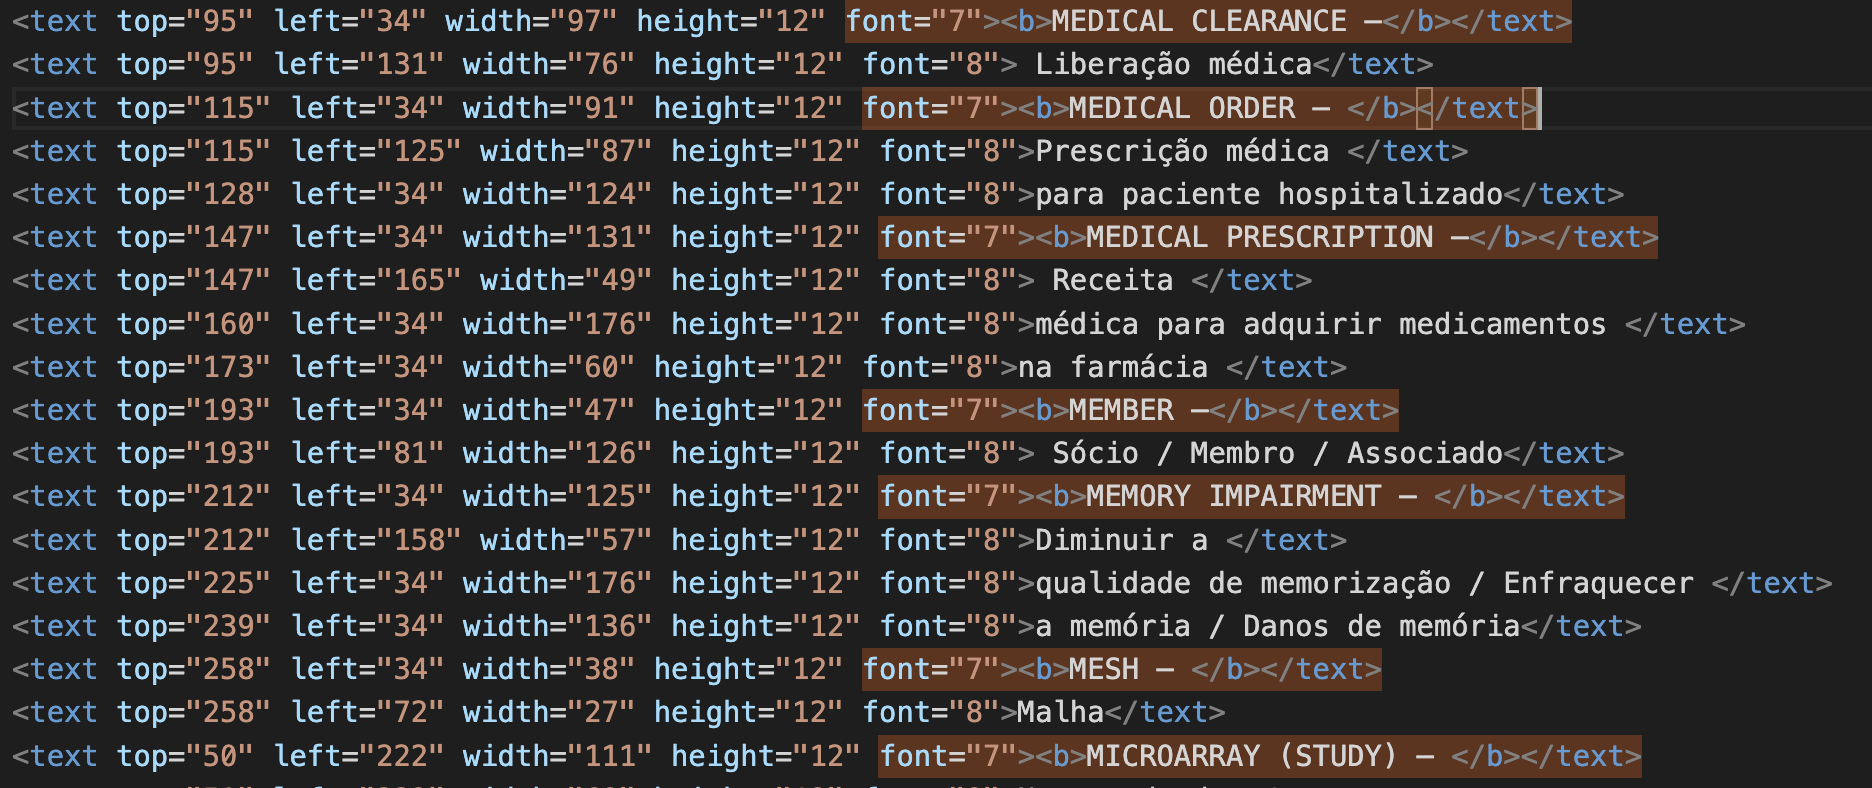
\includegraphics[width=\textwidth]{Images/padrao1.png}
      \caption{Padrão dos termos na secção Inglês-Português}
      \label{fig:padrao1}
    \end{subfigure}

    \begin{subfigure}{0.8\textwidth}
      \centering
      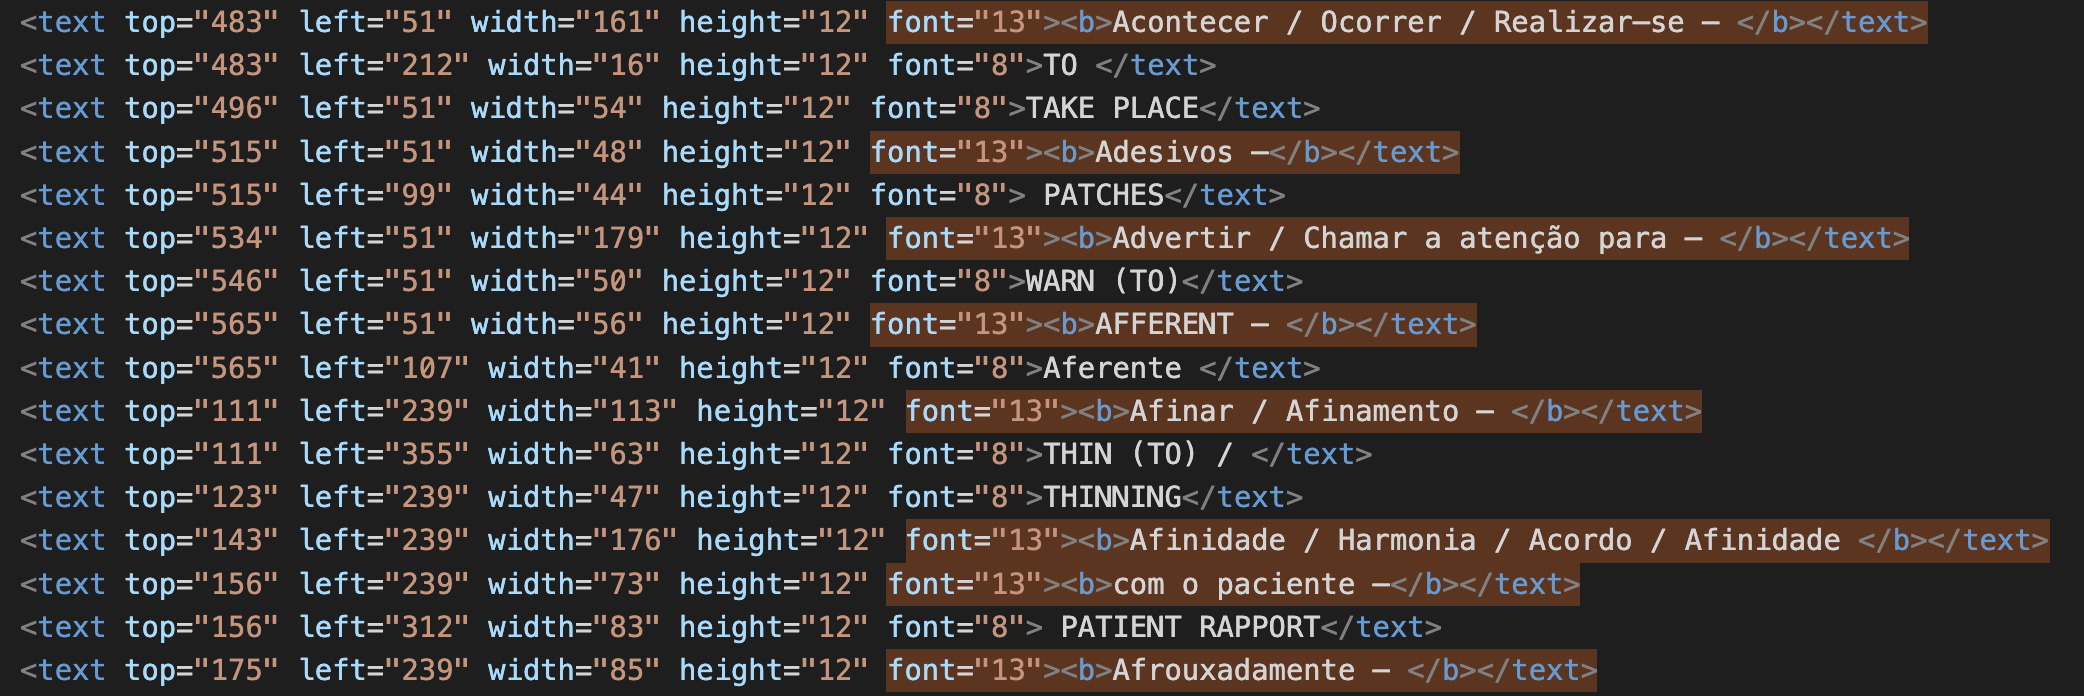
\includegraphics[width=\textwidth]{Images/padrao2.png}
      \caption{Padrão dos termos na secção Português-Inglês}
      \label{fig:portugues-ingles}
    \end{subfigure}
    \caption{Padrões observados em relação aos termos}
    \label{fig:termos}
\end{figure}

\begin{figure}[H]
    \centering
    \centering
    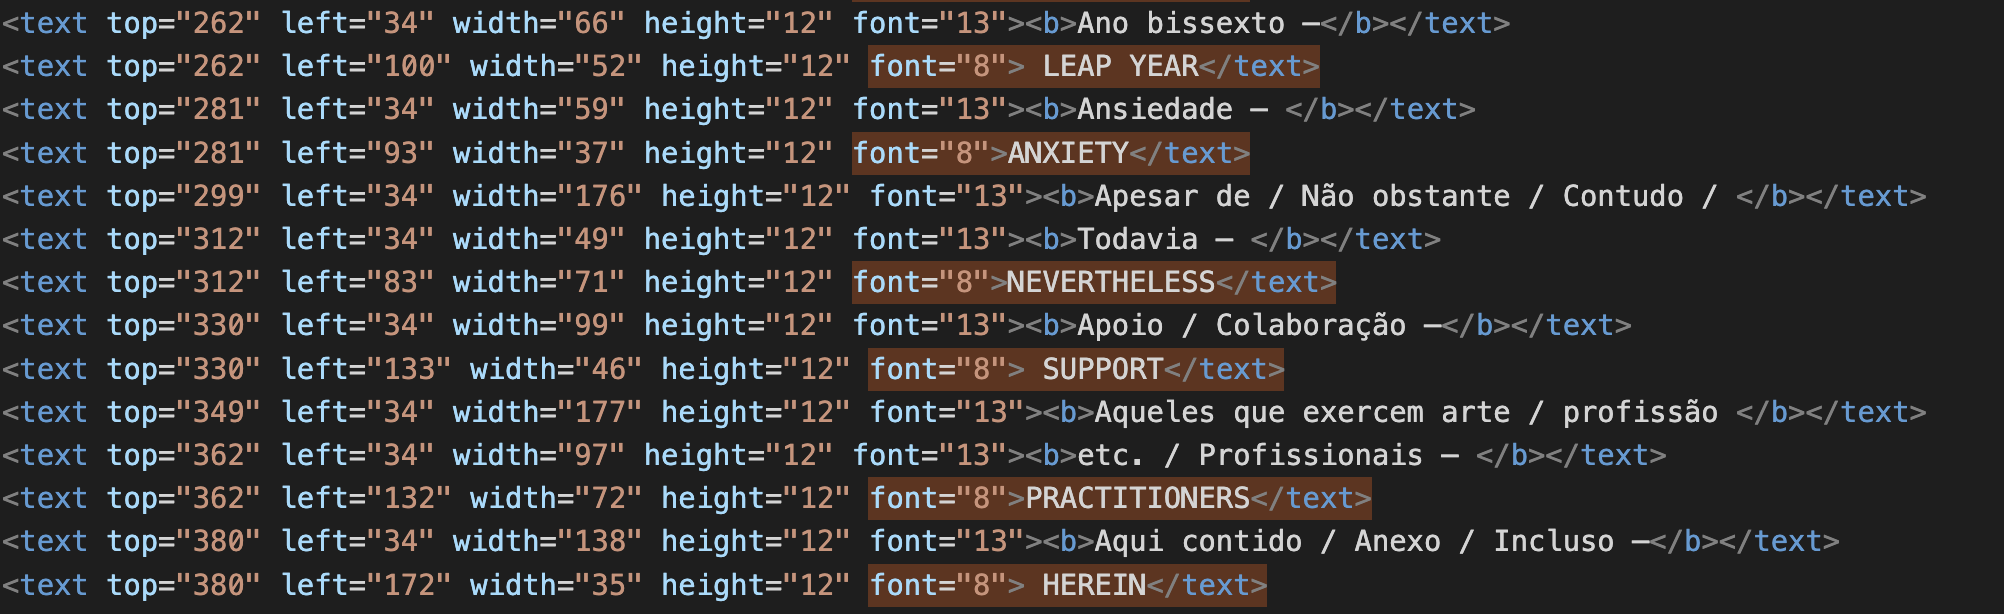
\includegraphics[width=0.8\textwidth]{Images/padrao3.png}
    \caption{Padrão observado em relação às traduções}
    \label{fig:traducoes}
\end{figure}

\subsubsection{Fase 3: Correção de anomalias}

Após a extração dos termos e traduções de acordo com os padrões identificados, foi possível observar que alguns elementos apresentavam erros devido à estruturação do ficheiro xml.

O termo \textbf{1st / 2nd / 3rd / 4th / SOUND} na secção Inglês-Português apresenta um padrão diferente dos demais: os identificadores de números ordinais \textbf{st}, \textbf{nd}, \textbf{rd} e \textbf{th} apresentam tags \textbf{<text>} com a propriedade \textbf{font="11"}. Na secção Português-Inglês, a respetiva tradução deste termo, em relação à propriedade \textbf{font}, possui valor 14. Portanto, para realizar uma correta extração, foi necessário adicionar condições \textbf{if} ao código desenvolvido em Python:

\begin{lstlisting}[style=pythonstyle]
if 'font="7"><b>' in line and ('font="7"><b>' not in previous_line and 'font="11"><b>' not in previous_line)
\end{lstlisting}

\begin{lstlisting}[style=pythonstyle]
if 'font="8">' in line and ('font="8">' not in previous_line and 'font="14">'not in previous_line)
\end{lstlisting}

\begin{lstlisting}[style=pythonstyle]
if 'font="8"' not in next_line and 'font="14">' not in next_line
\end{lstlisting}

Além disso, foi possível verificar que alguns elementos apresentam, entre o termo e a tradução, tags \textbf{<text>} sem conteúdo, o que também gera erros no processo de extração. Logo, foi realizada a devida eliminação através de uma condição \textbf{if} juntamante com a função \textbf{search} das RegEx:

\begin{lstlisting}[style=pythonstyle]
if re.search(r'font="8"> <.*', line)
\end{lstlisting}

\subsubsection{Fase 4: Construção do dicionário final}

Para a construção do dicionário final com a estrutura apresentada, foi necessário dividir as listas, citadas anteriormente, \textbf{lista\_termos} e \textbf{lista\_traducoes} em sublistas, porque, de acordo com a estruturação do documento, os primeiros 512 elementos de cada lista correspondem à secção Inglês-Português e, os demais, à secção Português-Inglês.

Após essa etapa, de maneira geral, o raciocínio consistiu em:

\begin{itemize}

    \item Definição de um dicionário, \textbf{dic\_traduc}, com as chaves \textbf{ingles-portugues} e \textbf{portugues-ingles}, para armazenar os dados extraídos em dicionários vazios;

    \item Para a chave \textbf{ingles-portugues}, foi adicionado ao seu dicionário vazio cada elemento da sublista \textbf{en\_pt\_termos} com a sua respetiva tradução presente na sublista \textbf{en\_pt\_traducoes};

    \item Em relação à chave \textbf{portugues-ingles}, foram adicionados os elementos (termos e traduções) que estavam armazenados nas sublistas \textbf{pt\_en\_termos} e \textbf{pt\_en\_traducoes} respetivamente;

    \item Após a inserção de todos os termos e traduções, o dicionário dic\_traduc é \textbf{convertido em formato JSON};

    \item O ficheiro final designa-se \textbf{"dic\_traduc.json"} com codificação UTF-8 e formato de indentação de 4 espaços.

\end{itemize}

\begin{figure}[H]
    \centering
    \centering
    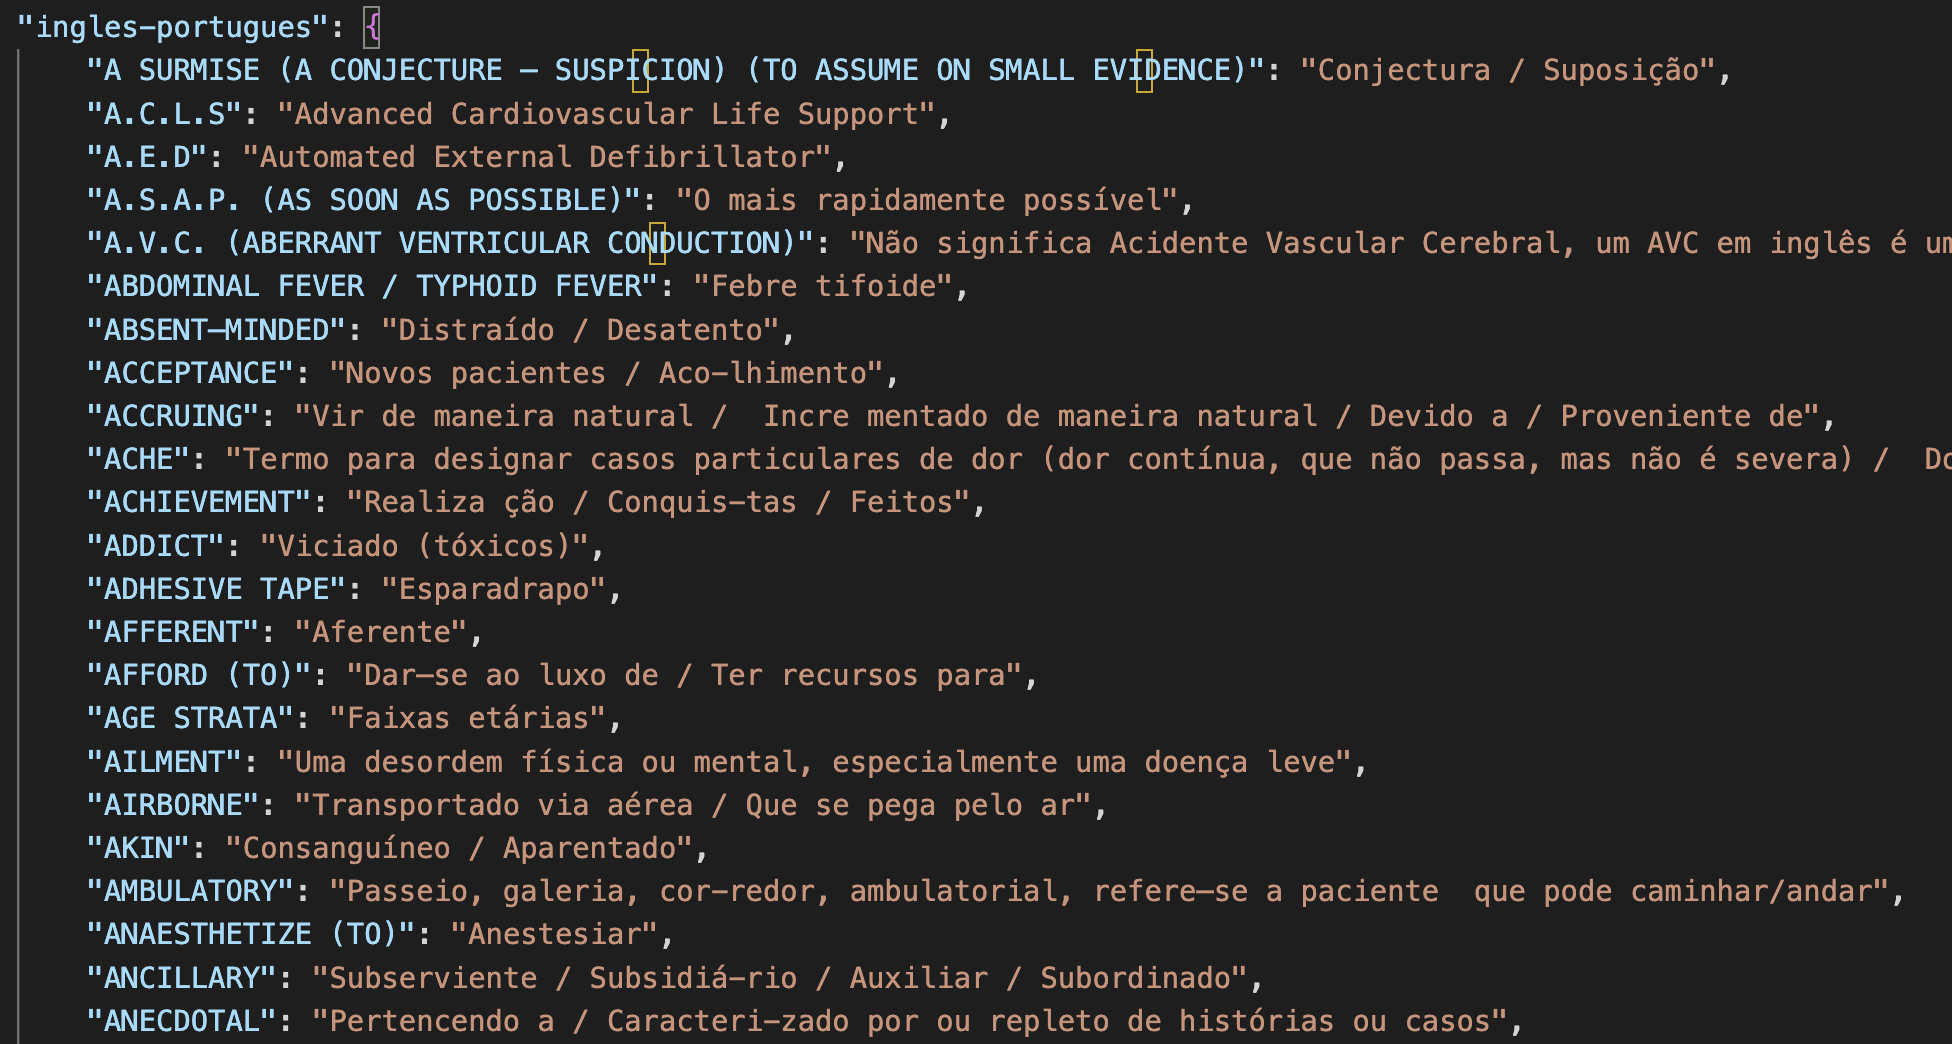
\includegraphics[width=0.8\textwidth]{Images/dic-traduc1.png}
    \caption{Secção Inglês-Português do dicionário final}
    \label{fig:dic-traduc1}
\end{figure}

\begin{figure}[H]
    \centering
    \centering
    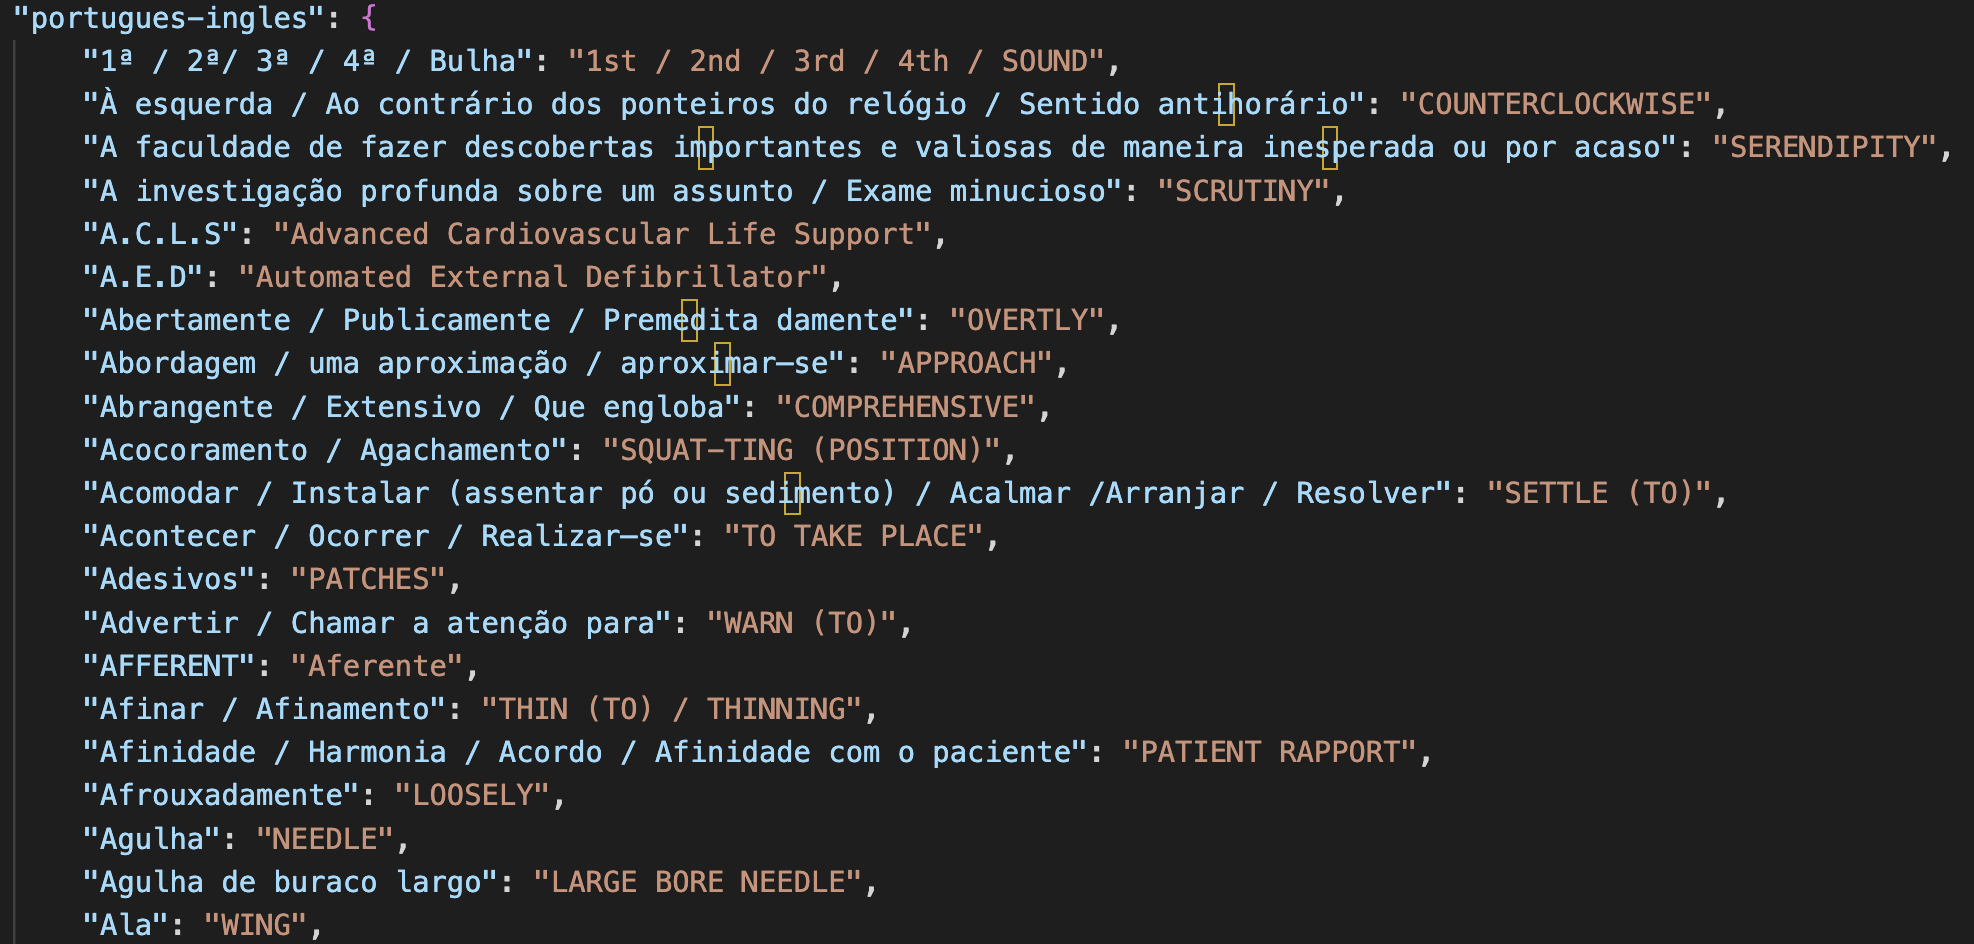
\includegraphics[width=0.8\textwidth]{Images/dic-traduc2.png}
    \caption{Secção Português-Inglês do dicionário final}
    \label{fig:dic-traduc2}
\end{figure}
